% !TeX root = ../main.tex

\chapter{神经辐射场的快速新视图合成方法研究}\label{citations}
上一章对本文研究相关的理论和技术进行了概述。本文的研究始终围绕着“基于神经辐射场的新视图合成加速”这一框架展开。本章主要详细介绍本文的方法论部分,包含问题的定义,NeRF 的相关预备理论,以及本文提出的对 NeRF 加速的具体方法,最后是对本章的总结。

\section{问题定义}
本节将简要阐述本文所研究问题的定义。
首先本文的研究目标是基于移动端相机采集的物体的不同视角的图像,快速渲染推理出新视角下的图像。要达到上述目标需要解决 NeRF 网络中如下的几个问题:
\begin{enumerate}
    \item 由于新视图合成是细粒度的渲染问题,NeRF 为了获取对渲染图象贡献较高的采样点,在训练和推理的过程中使用 coarse 网络和 fine 网络,通过 coarse 网络的输出来估计体密度随深度的变化分布,然后基于此分布进行二次采样并通过 fine 网络预测的颜色和体密度进行数值积分计算出 2D 图像对应像素的 RGB 值,这样两个网络的前向传播带来的开销是比较大的。
    \item NeRF 为训练更准确的神经辐射场,使用了深度学习网络,该网络本质上是逐点网络,受 justlookup\cite{lin2019justlookup}启发,同样可以使用查询表缓存其逐点网络的中间特征,对合成新视图的过程进行加速。
\end{enumerate}

\section{新视图合成的神经辐射场表示}
新视图合成的目的是基于已有的视角的图像,推理未知视角下的图像,现有的基于神经辐射场的体绘制方法已经可以合成较高质量的新视角图像。本节详细介绍神经辐射场 NeRF 的主要方法,包含神经辐射场的场景表示,基于神经辐射场的立体渲染,神经辐射场的优化三部分,由 NeRF 的方法论给本文提供一定的问题来源和理论支撑。

\begin{figure}[htbp]
    \centering
    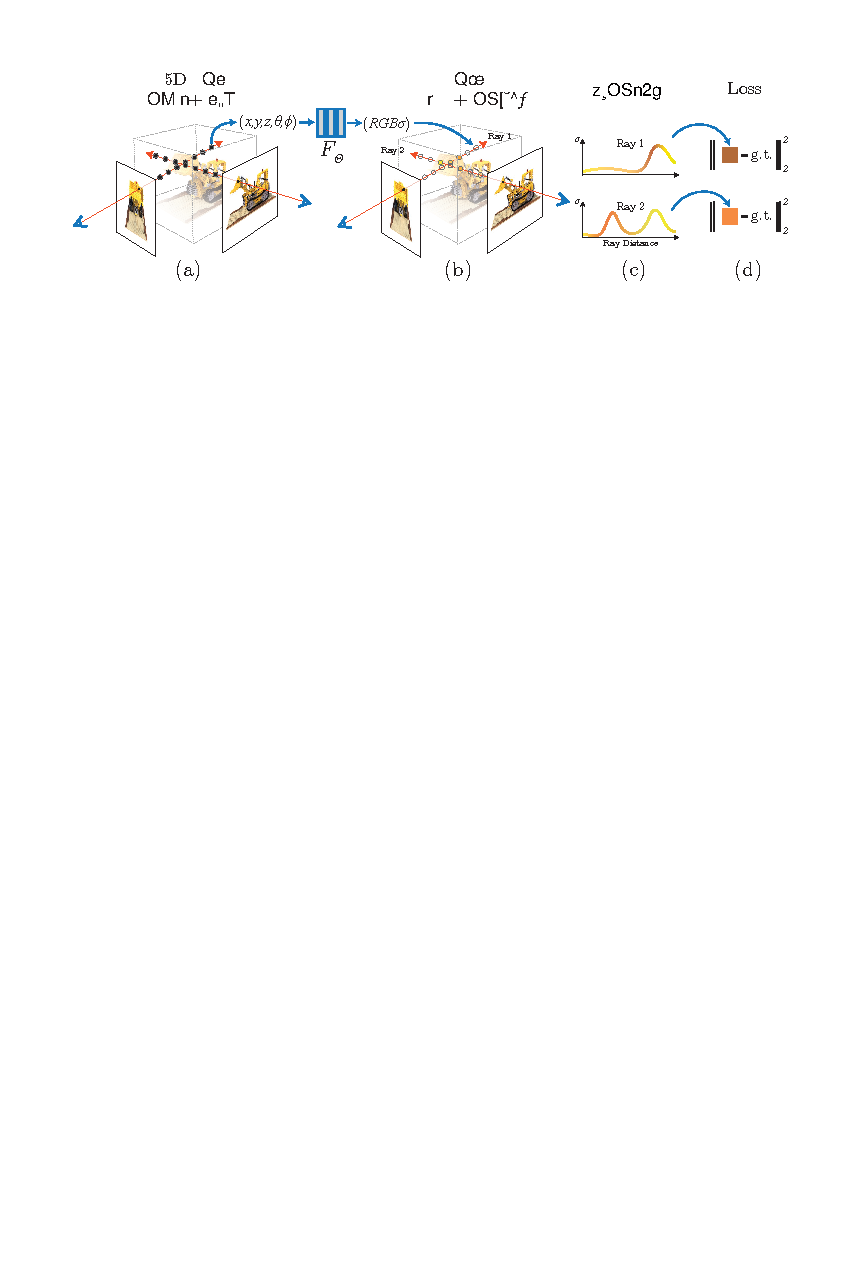
\includegraphics[width=0.95\linewidth]{figures/nerf_io.pdf}
    \caption{神经辐射场的场景表示和可微的渲染过程概况\cite{mildenhall2020nerf}。(a) 沿着相机光线采样 5D 坐标(位置和观测方向);(b) 将 (a) 中位置馈入 MLP 以生成颜色和体密度;(c) 将 (b) 中的这些输出使用立体渲染的方法合成相应的图像;(d) 此渲染过程是可微的,因此可以通过最小化合成的和 ground truth 观测图像之间的残差来优化场景表示。}
    \label{fig:nerf_io}
\end{figure}

\subsection{神经辐射场的场景表示}
如图~\ref{fig:nerf_io} 所示,NeRF 的整体框架是使用 5D 的向量值函数来表示连续的场景,其中,输入是一个 3D 坐标$\displaystyle \symbf{x} = \left(x, y, z \right)$ 和 2D 的视角方向 $\displaystyle \left(\theta, \phi \right)$,输出是发出的颜色$\displaystyle \symbf{c} = \left(r, g, b \right)$和体密度$\displaystyle \sigma$。实际上,方向被表示为三维直角坐标系中的单位向量$\displaystyle \symbf{d}$。NeRF 通过 MLP 网络$\displaystyle F_{\Theta} : \left(\symbf{x}, \symbf{d} \right) \Rightarrow \left(\symbf{c}, \sigma \right)$ 来估计这个连续的 5D 场景表示,并优化网络权重 $\displaystyle \Theta$ ,建立起 5D 坐标到相应的体密度以及相机光线方向发出颜色的映射,这是神经辐射场最基本的模型。下面将详细介绍基于神经辐射场的立体渲染的方法。

\subsection{基于神经辐射场的立体渲染}
NeRF 的 5D 神经辐射场将场景表示为空间内任意一点的体密度和定向发出的辐射,并且使用经典体积渲染的原理来渲染穿过场景的任何光线的颜色。体积密度$\displaystyle \sigma \left(\symbf{x} \right)$可以解释为一条光线在$\displaystyle \symbf{x}$位置处终止于无穷小粒子的概率。相机光线$\displaystyle \symbf{r}\left(t \right) = \symbf{o} + t \symbf{d}$在近远界限分别为$\displaystyle t_n$和$\displaystyle t_f$时所对应的颜色的期望为:
\begin{equation}
    C \left(\symbf{r} \right) = \int_{t_n}^{t_f}T\left(t\right)\sigma\left(\symbf{r}\left(t\right)\right)\symbf{c}\left(\symbf{r}\left(t\right), \symbf{d}\right)dt, 
    \textit{其中}T\left(t\right) = \exp \left(-\int_{t_n}^{t}\sigma\left(\symbf{r}\left(s\right)\right)ds\right).
\end{equation}
$\displaystyle T\left(t\right)$表示沿光线从$t_n$到$t$的累积透射率,即$t_n$到$t$光线没有碰到任何粒子的概率。从连续的神经辐射场中渲染一个视图需要为跟踪到期望虚拟相机的每一条相机光线估计积分$\displaystyle C\left(\symbf{r}\right)$。

计算机是无法计算连续积分的,因此需要使用数值估计的方法,利用求面积法估计连续积分。 确定性求面积通常用于渲染离散体素网格,将有效地限制所表示的分辨率,因为 MLP 仅在固定的离散位置上查询。 相反,NeRF 使用分层抽样方法将$\displaystyle \left[t_n, t_f\right]$放入$N$个均匀分布的容器中,然后从每个容器中随机抽取一个样本:
\begin{equation}
    t_i \sim U \left[t_n + \frac{i - 1}{N}\left(t_f - t_n\right), t_n + \frac{i}{N}\left(t_f - t_n\right) \right].
    \label{eq:uniform}
\end{equation}
虽然使用的是离散的样本集去估计积分,但是分层采样使其能表示连续的场景,这是因为它使得 MLP 在优化过程中可对连续的位置进行评估。 最终是通过这些样本来估计$C(r)$。
\begin{equation}
    \hat{C}\left(\symbf{r}\right)=\sum_{i=1}^{N}T_i\left(1-\exp\left(-\sigma_i\delta_i\right)\right)\symbf{c}_i, \textit{其中}T_i=\exp\left(-\sum_{j=1}^{i-1}\sigma_j\delta_j \right),
    \label{eq:getcolor}
\end{equation}
在公式~\ref{eq:getcolor} 中,$\displaystyle \delta_i = t_{i + 1} - t_i$是相邻两个采样点的距离。上述函数对于计算$\displaystyle \hat{C}\left(\symbf{r}\right)$的一组$\displaystyle \left(\symbf{c}_i, \sigma_i\right)$值是可微的,使用 alpha 值 $\displaystyle \alpha_i = 1 - \exp \left(-\sigma_i\delta_i\right)$ 可以简化成传统的 alpha 合成。 

\subsection{神经辐射场的优化}
上一节描述了将场景建模为神经辐射场的具体思路以及从该表示中渲染新视图所必需的核心组件。 但是,NeRF注意到这些组件不足以实现更高质量的神经渲染。NeRF介绍了两项改进,以此表示高分辨率的复杂场景。 第一种是输入坐标的位置编码,可帮助MLP表示高频函数,第二种是分层采样过程,可让有效地采样此高频表示。

\subsubsection{位置编码}
尽管理论上神经网络可以拟合任何函数,但是 NeRF 发现直接向网络$\displaystyle F_{\Theta}$中输入$\displaystyle xyz\theta\phi$会使得渲染效果不是非常好,在颜色和几何的高频变化上表现的非常差。这与 Rahaman 等人\cite{rahaman2019spectral}最近的工作是一致的,该工作表明深度学习网络倾向于学习低频函数。他们还表明,在将输入传递到网络之前,使用高频函数将输入映射到更高维度的空间可以更好地拟合包含高频变化的数据。

在神经场景表示的背景下利用上述发现,把$\displaystyle F_{\Theta}$重构成一个由两个函数组成的复合函数$\displaystyle F_{\Theta} = F_{\Theta}^{\prime} \circ \gamma$,$\displaystyle F_{\Theta}^{\prime}$是学习得到的,$\displaystyle \gamma$则是已知的,这能够明显地提升合成新视图的质量。$\displaystyle \gamma$建立了$\displaystyle \mathbb{R}$到更高维空间$\displaystyle \mathbb{R}^{2L}$的映射,$\displaystyle F_{\Theta}^{\prime}$仍是一个常规的 MLP。正式使用的编码函数如下:
\begin{equation}
    \gamma\left(p\right) = \left(\sin\left(2^{0}\pi p\right), \cos\left(2^{0}\pi p\right), \cdots, \sin\left(2^{L - 1}\pi p\right), \cos\left(2^{L - 1}\pi p\right)\right).
\end{equation}
$\displaystyle \gamma\left(\cdot\right)$函数作用于$\symbf{x}\left(\symbf{x} \in \left[-1, 1\right]^{3}\right)$的每个坐标值和$\displaystyle \symbf{x}$视角方向的单位向量$\displaystyle \symbf{d}$的每一个坐标值。

\subsubsection{分层体积采样}
接下来介绍一下 NeRF 中最核心的部分,分层体积采样。一般的渲染策略是,在每条相机光线上密集地采样$N$个查询点,然后通过神经辐射场网络去评估得到颜色和体密度,但是这一渲染策略效率十分低下:自由空间和对渲染图像无贡献的遮挡区域仍会被重复采样。 NeRF 从体绘制中的早期工作\cite{levoy1990efficient}中汲取灵感,并提出一种分层表示,通过按比例分配样本到最终渲染的预期效果来提高渲染效率。

NeRF 同时优化两个神经网络:一个是 coarse 网络,另一个是 fine 网络。首先使用分层采样采集一组有$N_c$个位置的样本,在这些位置使用公式~\ref{eq:uniform} 和公式~\ref{eq:getcolor} 来评估 coarse 网络。基于这个 coarse 网络的输出,就可以沿着每条光线对点进行更准确的采样,此时的样本点更偏向于物体附近。为此,首先将公式~\ref{eq:getcolor} 中的 coarse 网络$\displaystyle \hat{C}_{c} \left(\symbf{r}\right)$的alpha合成颜色重写为沿射线的所有采样颜色$\displaystyle c_i$的加权和:
\begin{equation}
    \hat{C}_{c}\left(\symbf{r}\right) = \sum_{i=1}^{N_c}w_{i}c_{i}, w_{i} = T_{i}\left(1 - \exp \left(-\sigma_{i}\delta_{i}\right)\right).
    \label{eq:weight}
\end{equation}
将上述权重进行归一化$\displaystyle \hat{w}_{i} = \frac{w_i}{\sum_{j=1}^{N_c}w_j}$可以生成一个沿着相机光线分段常数的概率密度函数。我们使用逆变换采样从该分布中采样第二组$\displaystyle N_f$个位置,最终使用公式~\ref{eq:getcolor} 来计算最终沿着光线渲染的颜色,此时使用所有$\displaystyle N_c + N_f$个采样点。

由于优化的是两个网络,因此对于一个 batch 的光线集合$\mathcal{R}$,整个 NeRF 的 loss 可以表示为:
\begin{equation}
    \mathcal{L} = \sum_{\symbf{r}\in \mathcal{R}}\left[\left\|\hat{C}_{c}\left(\symbf{r}\right) - C\left(\symbf{r}\right)\right\|_{2}^{2} + \left\|\hat{C}_{f}\left(\symbf{r}\right) - C\left(\symbf{r}\right)\right\|_{2}^{2} \right].
    \label{eq:nerf_loss}
\end{equation}
这个也是本文的研究动机,通过优化上述的采样过程,使 NeRF 可以减少训练一个网络,这是本文最核心的改进思想。

\section{基于神经辐射场的新视图合成加速方法}\label{method}
针对 NeRF 采用分层抽样这一做法,即同时优化 coarse 网络和 fine 网络,通过 coarse 网络的输出去估计公式~\ref{eq:weight} 中的权重$\displaystyle w_i$的分布情况,生成一个分段常数的概率密度函数,通过此分布进行二次采样并馈入 fine 网络中,这在 NeRF 中证明是能显著提升渲染质量的。但也正是由于增加了一个网络,那么在网络前向传播这一部分的开销增加了一倍,这在实际应用中是难以接受的。为此,本文将此问题看作是一个领域知识的优化的问题。优化的目标在于无论是训练还是在测试过程中,只使用一个网络,这样理论上渲染一张新视图的时间会缩短一半。但是,在 NeRF 消融实验中证明了单纯地使用一个网络势必会降低新视图渲染的质量,因此必须采取一定的方式去补偿减少一个网络带来质量下降的问题。接下来首先会介绍本文提出的一个最基本的加速优化模型;然后详细介绍该模型中的核心组件查询表的构建,其中包含网络架构和如何建立对查询表的快速索引。

\subsection{模型综述}
本小节将详细介绍本文提出模型的设计方法和细节。
\begin{figure}[t]
    \centering
    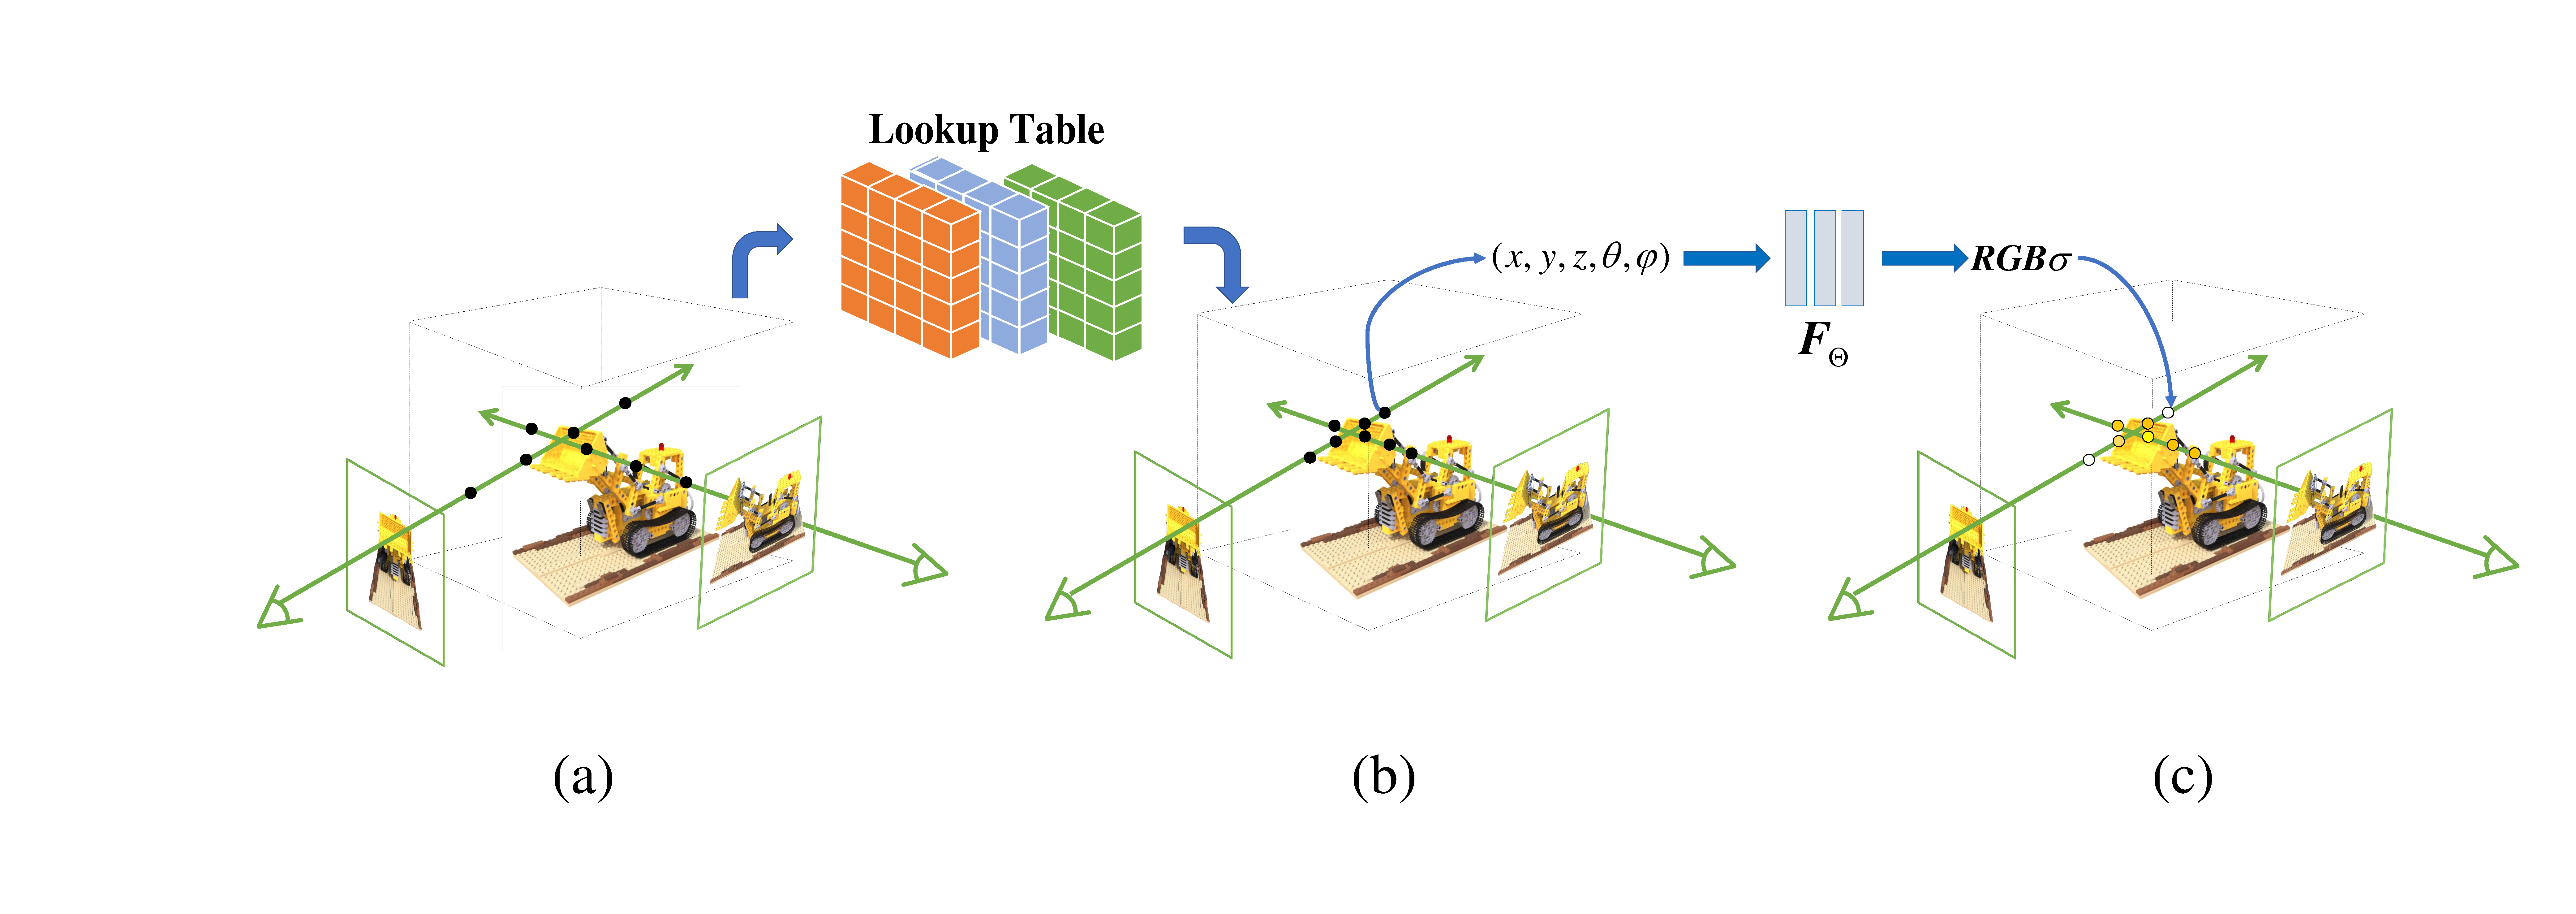
\includegraphics[width=0.95\textwidth, height=0.25\textheight]{figures/fnerf.pdf}
    \caption{神经辐射场的新视图合成的加速框架。(a) 沿着相机光线采样 5D 坐标(位置和观测方向);(b) 通过缓存的特征查询表找到采样点中距离表面最近的点,并在此点附近进行二次采样;(c) 将 (b) 中位置$\left(x, y, z\right)$和方向$\left(\theta, \phi\right)$馈入 MLP 以生成颜色$RGB$和体密度$\sigma$。}
    \label{fig:fnerf}
\end{figure}
如图~\ref{fig:fnerf} 所示,本文提出了基于神经辐射场的快速合成新视图的框架,为 NeRF 的推理过程进行加速。本文的框架一共包含以下三个步骤:
\begin{enumerate}
	\item 减少网络 \\
	对于减少网络来说,由于 NeRF 是使用了 coarse 网络和 fine 网络来进行分层采样,为了操作方便,本文是去掉了 coarse 网络,仅保留 fine 网络,这显然会降低渲染的质量水平,因此还需要后面两个步骤的操作。
	\item 提取查询表 \\
	对于缓存查询表的过程,由于场景是有限的,可以限制在立方体中,然后将立方体体素化,将格点坐标输入到 NeRF 预训练好的网络中,根据体密度为正值这一条件筛选出场景内部点的坐标,查询表真正存的是网络中间层(第四层的输出)的特征,查询表实质表征了物体的近似表面,具体的查询表的构建详见下一小节。
	\item 优化采样 \\
	通过缓存的查询表完成对采样点的优化,过程的概况为首先将粗采样的采样点(均匀采样完成的)馈入查询表中,若发现光线上所有点均不在查询表内则忽略该条光线,下面是有交集的情况,沿着光线的方向找到相机光线上第一个在查询表内的点,以此点为中心,适当的区间长度进行二次均匀采样,这些采样点即最终的采样点,位于物体表面附近,对渲染图像贡献较大。之后将高贡献的采样点馈入 NeRF 原有的网络框架(即 fine 网络)中输出颜色和体密度,通过积分计算出像素的 RGB 值,然后可以根据该 RGB 值与 ground truth 对应像素的 RGB 计算出 loss 并反向传播优化整个网络。
\end{enumerate}            
%对于网络裁剪来说,由于 NeRF 是使用了 coarse 网络和 fine 网络来进行分层采样,为了操作方便,本文是去掉了 coarse 网络,仅保留 fine 网络,这显然会降低渲染的质量水平,因此还需要后面两个步骤的操作。对于缓存查询表的过程,这里先简单理解为建立了一个立方体网格,将格点坐标输入到 NeRF 预训练好的网络中,根据体密度为正值这一条件筛选出场景内部点的坐标,查询表真正存的是网络中间层(第四层的输出)的特征,查询表实质表征了物体的近似表面,具体的查询表的构建详见下一小节。对于第三步,我们通过缓存的查询表完成对采样点的优化,过程的概况为首先将粗采样的采样点(均匀采样完成的)馈入查询表中,若发现光线上所有点均不在查询表内则忽略该条光线,下面是有交集的情况,沿着光线的方向找到相机光线上第一个在查询表内的点,以此点为中心,适当的区间长度进行二次均匀采样,这些采样点即最终的采样点,位于物体表面附近,对渲染图像贡献较大。之后将高贡献的采样点馈入 NeRF 原有的网络框架(即 fine 网络)中输出颜色和体密度,通过积分计算出像素的 RGB 值,然后可以根据该 RGB 值与 ground truth 对应像素的 RGB 计算出 loss 并反向传播优化整个网络,最后我们就获得了一个能快速合成新视图的网络框架。

\subsection{查询表的构建}
\begin{figure}[t]
    \centering
    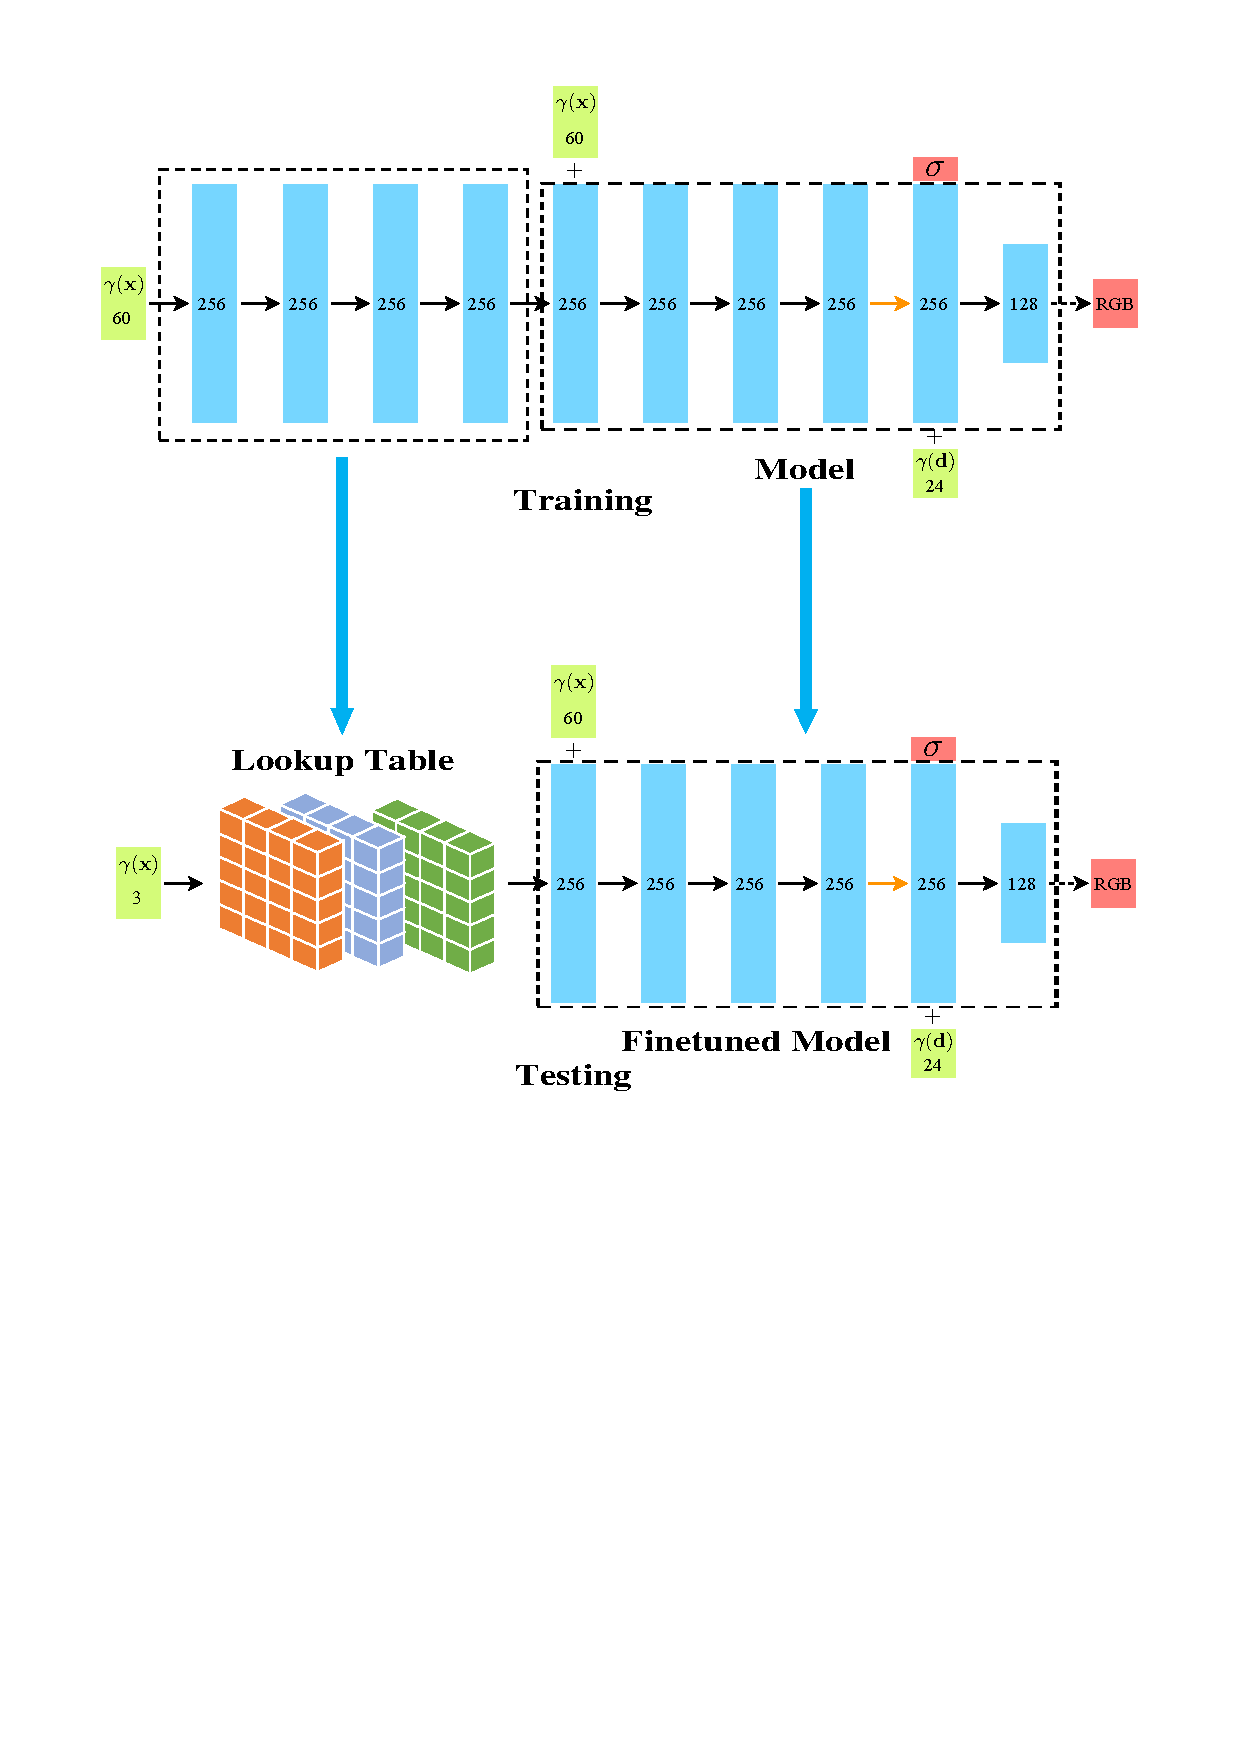
\includegraphics[width=0.95\textwidth]{figures/lookuptable.pdf}
    \caption{查询表的构建以及类似justlookup\cite{lin2019justlookup}的架构,通过缓存网络特征来进行加速,并通过重新训练的方法对近似的特征进行学习。}
    \label{fig:lookuptable}
\end{figure}

本节将详细介绍前一节中查询表的构建,主要介绍查询表的数据类型,生成方式,快速索引的方法,以及如何压缩 NeRF 的网络。

如图~\ref{fig:lookuptable} 所示,本文主要的构建方法是首先训练一个逐点网络,即使用 NeRF 的原网络进行预训练,将网络的前四层全连接层提取出来,我们可以得到一个逐点函数$\mathcal{G}$,类似justlookup\cite{lin2019justlookup},我们使用查询表技术并利用数组索引的方法能够快速地获得近似的函数$\hat{\mathcal{G}}$。

详细地,由前面的理论可知,我们可以用相机光线$\symbf{r}\left(t\right) = \symbf{o} + t \symbf{d}, t \in \left[t_n, t_f\right]$表示一组采样点的集合,为了使用方便,事先对光线的坐标范围进行尺度缩放,使得
$\forall t \in  \left[t_n, t_f\right], \symbf{r}\left(t\right) \in \left[-1, 1\right]^3$。

为表示方便,先忽略位置编码函数$\gamma\left(\cdot\right)$的作用,假设逐点网络输入的是三维坐标点,那么可以将上述的映射$\mathcal{G}$表示为$\mathcal{G}: \mathbb{R}^3 \Rightarrow \mathbb{R}^l$, 其中$l$在是第四层全连接网络输出变量的个数,在本文中$l = 256$。更具体地,$\mathcal{G}$是由四层 MLP 实现的,每一层的输出的数目均是256。

为了学习$\mathcal{G}$,我们利用原网络剩下的部分记为 Model 。使用公式~\ref{eq:nerf_loss} 中的均方误差联合优化这个端到端的网络,最终得到三元函数$\mathcal{G}$。一旦我们获得了$\mathcal{G}$,我们就可以通过构建一个查询表来获得近似的函数$\hat{\mathcal{G}}$。

显然,我们现在的最重要的一步是为$\mathcal{G}$构建查询表。为了方便,我们还是假设输入被缩放到一个固定大小的立方体$\mathcal{V}$里,其中$\mathcal{V} = \left[-1, 1\right]^3$。接着将$\mathcal{V}$分成规则的$M^3$个相等的体素块。那么每一个体素的边长则为$\Delta = \frac{2}{M}$。
% 那么因此立方体$\mathcal{V}$则被分成了:
% \begin{equation}
%     \mathcal{V} = \bigcup_{i,j,k}\left[i\Delta, \left(i + 1\right)\Delta\right] \times \left[j\Delta, \left(j + 1\right)\Delta\right] \times \left[k\Delta, \left(k + 1\right)\Delta\right], \mbox{其中} \left(i, j, k\right) \in \left[0, M\right]^3.
% \end{equation}

区别于justlookup\cite{lin2019justlookup},我们并没有采取$T\left[i\right]\left[j\right]\left[k\right] = \mathcal{G}\left(i\Delta, j\Delta, k\Delta\right), \left(i, j, k\right) \in \left[0, M\right]^3$,即存下所有格点所对应的特征,这样在 NeRF 这样细粒度的渲染工作中几乎是不可取的。实际中,我们需要使用 float32 的数据类型去存储,那么总内存开销就会达到$32M^{3}l bits$,以$l = 256, M = 256$为例,则需要$\SI{16}{GB}$的内存,随着查询表的边长$M$增加,内存是以三次方的速度在增长,这在实际操作中是不可行的。

\begin{figure}[b]
    \centering
    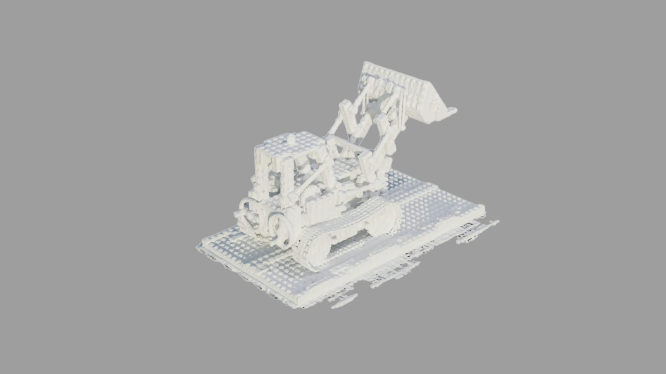
\includegraphics[width=0.95\textwidth]{figures/legomesh_gray_complete.png}
    \caption{使用 NeRF 网络(体密度 $> 0$)提取出的 lego 的 mesh 结构}
    \label{fig:lego_mesh}
\end{figure}

为此,我们必须采取相应的措施去压缩查询表。受 DeepSDF \cite{park2019deepsdf}的启发,在 DeepSDF 这篇工作中,可以通过输出的 SDF 值,利用 marching cubes 算法\cite{lorensen1987marching}重建物体的几何结构,类似地,我们知道 SDF 的物理含义是某一三维坐标点到物体表面的最短距离,负值表示在物体内部,正值表示在物体外部,零值则是物体表面;那么,NeRF 输出的体密度信息也有着相似的性质,体密度的物理含义是相机光线终止于某一点的概率,那么同样地,体密度为零值也可以表征物体的表面, 图~\ref{fig:lego_mesh} 就是用 NeRF 模型提出 lego 的 mesh 结构。根据公式~\ref{eq:weight} 可以看出当体密度为负值时权重$w_i$是负值是没有意义的,这也与 NeRF 的处理方式相同,NeRF 在体密度输出的时候使用了 ReLU 函数,因此我们可以认为负值的体密度对渲染的贡献可以忽略。那么结合上一节,如果我们可以将采样点约束在物体表面附近,那么将能获得更好的渲染效果,这可以补偿减少一个网络带来的质量下降。

基于以上的分析,我们假设正值的体密度表征物体的内部,接下来就可以对原查询表进行压缩。我们的目标是只存$\mathcal{V}$中输出的体密度大于零的格点,这样可以大大减少内存的开销。

具体地,我们记从三维坐标点到输出体密度这一部分网络对应的函数为$\mathcal{Q}$,此时压缩后的查询表为:
\begin{equation}
    T_{shrinked} = \left\{
    \mathcal{G}\left(i\Delta, j\Delta, k\Delta\right) | \mathcal{Q}\left(i\Delta, j\Delta, k\Delta \right)  > 0, \left(i, j, k\right) \in \left[0, M\right]^3 
    \right\}.
\end{equation}
至此,我们获得了最终的查询表,由于此查询表是不规则的,或者可以认为是稀疏矩阵,因此索引此查询表也跟常规的方法不同,接下来将详细介绍经过压缩后的查询表的索引。

对于$ T_{shrinked}$ 的存的每一个格点$\left(i\Delta, j\Delta, j\Delta\right)$, 我们必须将每一个常规索引$\left(i, j, k\right)$ encode 到一个唯一值 code ,换句话说,我们的目标是使得$\mathcal{V}$中的任何一个格点对应的code都是不重复的。为此,我们可以使用以下的映射方式:
\begin{equation}
    \mathcal{E}\left(i, j, k\right) = i + j\cdot M + k\cdot M \cdot M, \left(i, j, k\right) \in \left[0, M\right]^3,
\end{equation}

这个对索引的编码操作可以使得将$\mathcal{V}$中的所有格点都区分开。

接下来,我们将建立一个 code 到 $T_{shrinked}$的查询表$\mathcal{H}$,。具体的建立方式为,
\begin{enumerate}
    \item[a)] 首先建一个大小$size = M + M^2 + M^3$的查询表$\mathcal{H}$,使之能装下$\mathcal{V}$中所有格点;
    \item[b)] 按照$T_{shrinked}$对应的所有点的顺序,假设其中一个点对应的常规索引为$\left(i, j, k\right)$,该点在$T_{shrinked}$的位置为$index$对其使用 encode 操作得到$code = \mathcal{E}\left(i, j, k\right)$;
    \item[c)] 之后填充查询表$\mathcal{H}$,具体做法是$\mathcal{H}[code] = index$。
\end{enumerate}
严谨来说,非$T_{shrinked}$的点在索引时,其$code$ 可能会超过$T_{shrinked}$的索引范围,因此,我们必须处理此问题。具体做法是,在$T_{shrinked}$的最后面加一个哨兵,即增加一个$l$维的全零的向量,假设目前$T_{shrinked}$存了$S$个点对应的特征。而$\mathcal{H}$在初始化的时候,初始值都设置为$S-1$,即当$\left(i, j, k\right)$不在查询范围内时,其$code$可以通过$\mathcal{H}$映射到$S-1$,那么将获取$T_{shrinked}\left[S-1\right]$的值,从而得到一个鲁棒的索引过程。

至此,我们可以总结整个索引的过程。给定一个空间直角坐标系的三维坐标点$\left(x, y, z\right)$,首先通过下面式子计算其常规索引:
\begin{equation}
    \left(i, j, k\right) = \left(\left \lfloor \frac{x + 1}{\Delta} \right \rfloor, \left \lfloor \frac{y + 1}{\Delta} \right \rfloor, \left \lfloor \frac{z + 1}{\Delta} \right \rfloor\right),
\end{equation}

有了常规索引后,需要对其进行 encode ,得到 $code = \mathcal{E}\left(i, j, k\right)$,之后通过 $\mathcal{H}$ 查询到 $code$ 对应的在$T_{shrinked}$中的索引,则整个查询过程为:
\begin{equation}
    T\left[i \right]\left[j \right]\left[k \right] = T_{shrinked} \left[\mathcal{H}\left[\mathcal{E}\left(i, j, k\right) \right] \right].
\end{equation}

最终,如果我们提前缓存了$T$,则可以使用$T\left[i \right]\left[j \right]\left[k \right]$的值去估计$\hat{\mathcal{G}}\left(x, y, z\right)$,因此$\hat{\mathcal{G}}$的将是非常快的,它的开销只取决于访问内存的时间。

显然,我们直接将$\hat{\mathcal{G}}$馈入到经过训练的模型 $Model$中会使渲染效果下降的,因为$\hat{\mathcal{G}}$并不完全正确
等于$\mathcal{G}$,$\hat{\mathcal{G}}$仅仅是$\mathcal{G}$的一个近似。因此为了保持渲染质量不下降,我们在构建了查询表$T$后,需要基于$\hat{\mathcal{G}}$对$Model$进行再训练(或着叫微调),这一操作能显著提升渲染质量,在$M = 200$的时候甚至可以达到和原始 NeRF 质量相当的性能。图~\ref{fig:lookuptable} 表征了$\mathcal{G}$是如何由我们的方法实现的。

\subsection{查询表与本文方法的结合}
我们在上一小节详尽地叙述了查询表的创建过程,包含查询表的构建,索引,压缩,还有通过近似$\mathcal{G}$来进行加速,通过再学习将损失的质量调回原 NeRF 水平。接下来,本节将详细介绍查询表的第二重加速功能:将查询表应用于 NeRF 的采样过程。

如果只是使用查询表去近似$\mathcal{G}$,那么这并没有完全展现出本文最核心的方法。实际上,在上一小节中,我们不止做了这么多工作。我们都知道,在查询表的构建过程中,本文是对查询表进行了压缩的操作,这表面上只是为了减少查询表内存开销,事实上我们还应用了 NeRF 体密度的特性。

由于我们是使用的体密度$\sigma > 0$这一阈值条件对$\mathcal{V}$中格点进行筛选,仅在$T_{shrinked}$中保留其体密度为正值的点所对应的特征(即$l$维向量),并且我们还在$T_{shrinked}$的最后放置了哨兵来表征没有查询到相应点的特征。

因此,我们可以合理地使用$\mathcal{H}$和$T_{shrinked}$这两个查询表对输入的点进行判断,显然如果可查询到,则该点在物体内部,否则不在物体内部。具体地,由于设置了哨兵,我们实际可以只使用索引转换查询表$\mathcal{H}$对内外进行判断。对于任意的常规索引$\left(i, j, k\right) \in \left[-1, 1\right]^3$,计算$\mathcal{H}\left[\mathcal{E}\left(i, j, k\right)\right]$的查询结果,若结果为$S - 1$,则原世界坐标$\left(x, y, z\right)$则不在物体(场景)的内部,若结果不为$S - 1$,则在物体内部。

\begin{figure}[t]
    \centering
    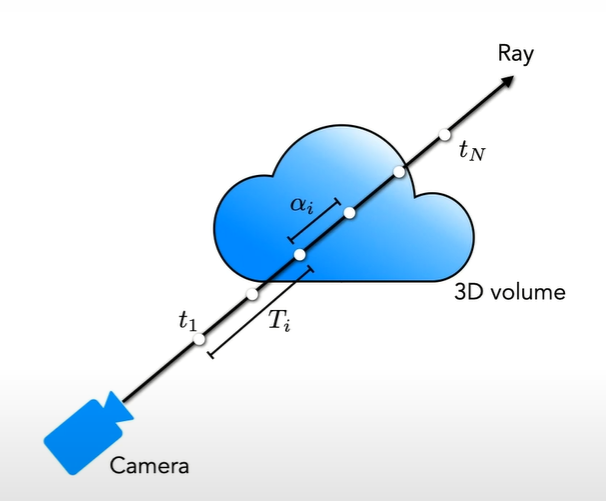
\includegraphics[width=0.95\textwidth]{figures/cloud.jpg}
    \caption{体绘制的采样示意图}
    \label{fig:cloud}
\end{figure}

有了以上的理论基础,接下来将详尽阐述是如何利用查询表进行采样优化以及加速。

针对前面两节的概述,我们知道,NeRF 是采用分层抽样的方法,即同时优化 coarse 网络和 fine 网络,通过 coarse 网络的输出去估计公式~\ref{eq:weight} 中的权重$\displaystyle w_i$的分布(概率密度函数),这是通过增加网络来提高渲染质量的方法。但同时也很显然,使用两个网络,那么时间开销会增加一倍。

为了加速 NeRF ,我们的目标是去掉一个网络,仅使用一个网络来进行优化和渲染,但是这势必会使得渲染质量下降。考虑到 NeRF 使用两个网络是为了将采样点位置优化到物体周围,这一点启发了我们,如果使用上述的查询表将采样点约束到物体表面附近,那么渲染质量会比仅使用一个网络显著提升,通过实验证明本文的方法可以在几乎不损失渲染质量的情况下对 NeRF 的推理过程进行加速。下面是查询表是如何和本文方法进行融合的。

如图~\ref{fig:cloud} 所示的是体绘制的采样示意图。假设相机光线为$\symbf{r}\left(t\right) = \symbf{o} + t \symbf{d}$,并在$\left[t_n, t_f\right]$的范围内均匀采样$N$个点,深度记为$t_{1}, t_{2}, \cdots, t_{N}$,这些深度是递增的,对应的点的世界坐标为$\symbf{r}\left(t_{1}\right), \symbf{r}\left(t_{2}\right), \cdots, \symbf{r}\left(t_{N}\right)$。分别计算这些点的常规索引,以及编码之后的 code,通过这些 code 去查询$\mathcal{H}$,得到一个长度为$N$的 vector。之后按顺序对 vector 的每一个坐标值进行判断,若值均为$S - 1$,则说明该光线与物体没有交点,则采样点不需要优化,若存在值不为$S - 1$的,则说明光线和物体有交点,记第一个交点对应的深度值为$t_{mid}, mid \in \left\{1, 2, \cdots, N\right\}$。在有交点的情况下,我们需要重新设定采样区间长度为$L$,则新的采样区间为$\left[t_{mid} - L / 2, t_{mid} + L / 2\right]$,此区间能表征物体的表面附近,我们需要在此区间内重新均匀采样$N$个点,${t\prime}_{1}, {t\prime}_{2}, \cdots, {t\prime}_{N}$,然后就可以将$\symbf{r}\left(t\prime_{1}\right), \symbf{r}\left(t\prime_{2}\right), \cdots, \symbf{r}\left(t\prime_{N}\right)$这些采样点送入网络进行训练,最终实验证明使用了改进的采样方式,在我们减少一个网络的时候,可以保证渲染质量几乎不下降。

最终,我们通过缓存一个查询表,成功地在不损失精度的情况下减少了一个网络的开销,对渲染过程进行了加速,那么因此,本文方法对应的 loss 函数变为:
\begin{equation}
    \mathcal{L} = \sum_{\symbf{r}\in \mathcal{R}}\left[\left\|\hat{C}\left(\symbf{r}\right) - C\left(\symbf{r}\right)\right\|_{2}^{2} \right].
    \label{eq:fnerf_loss}
\end{equation}

\section{本章小结}
本章首先介绍了本文所研究的问题定义。接着介绍了新视图合成任务中的神经辐射场表示方法,然后在此基础上详细地介绍了本文基于问题而提出的方法论,包含模型网络结构,查询表技术的引入与查询表的构建,以及如何把查询表应用到本文的方法中。

综上,本文借助查询表技术替换了一部分网络(逐点网络)参数,使得查询可以直接从内存(或缓存)中获取中间层的特征,这可以显著加速渲染过程;为了减少查询表的内存开销,同时也是为了与本文方法进行融合,我们对查询表进行了压缩的操作,具体是使用体密度$\sigma > 0$这一阈值条件去筛选位于物体内部的格点;本文的核心方法是减少 NeRF 的原始的两个网络的结构,我们仅采用一个网络进行训练和渲染,为了保证质量不下降,使用查询表判断原始采样点并第一个在物体内的点,并在此附近进行重新的均匀采样,可以补偿只用一个网络带来的质量下降;当然,最关键的一点是,将上述方法结合在一起时,由于查询表替换网络这一部分是用的近似特征,因此为了保证质量不下降,必须进行近似特征再学习。最终,通过本文的方法可以实现在几乎不损失精度的情形下对 NeRF 合成新视图进行加速。

\cleardoublepage
